\chapter{Open Loop Experiments}
The open loop experiments aim to verify the hypothesis that the human response to a robot handshake can be modelled as a dynamical model. In these experiments human participants are intended to be a natural calibration system for the robot grasping force $F_r$. The hypothesis on participant's grasping force is shown in \ref{EQ:forceSteady}, participants are asked to apply the force that they are perceiving during the experiments.
\begin{equation}
F_{h} = F_{r}
\label{EQ:forceSteady}
\end{equation}
this introduces a limitation on the evaluation of the data, in fact the equation is assumed to hold only in quasi-static systems. A procedure to filter the transient from the data is applied in order to evaluate the relation $q$ vs. $F_h$ when steady states are reached.
Force is exchanged during a handshake only after the reference position has reach the first contact point $q_0$, therefore for values of $q < q_0$ no force will be exchanged in the handshake. The constraints on $q$ introduced in \ref{sec:softhand} are valid through all this work since are hardware related.
The \textit{sensorized palm} is used in order to seek the force behaviour for values of the reference position $q > q_0$. The shells of the device are not deformable, due to the material used during the 3D printing. Increasing the reference position $q$ of the Pisa/IIT SoftHand squeezing the \textit{sensorized palm} showed a linear relationship between the difference $q-q_0$ and $F_r$, as	 
%\textcolor{magenta}{talk about why the spring relation is choosed}

\begin{equation}
F_{r}(q)=\left\{\begin{matrix}
k_{r}(q-q_0) & $ for $ &q-q_0 \geq 0 \\ 
0 & $ for $ & q-q_0 < 0
\end{matrix}\right.
\label{EQ:genericForce}
\end{equation}\\

%
%$$
%F_{r} = 
%  \begin{cases} 
%    $Dynamic to find$ & q-q_0 \geq 0 \\
%    0 & q-q_{0} < 0
%  \end{cases}
%$$\\

Where $F_r$ is the force during the handshake applied by the robot on the \textit{sensorized palm}, $q$ is the reference position sent to the device, $q0$ is the first contact point and $k_{r}$ is a constant parameter to seek.
During these experiments each reference position of the Pisa/IIT SoftHand is held for 3 seconds, the frequency rate of is set to 100Hz. \\
A file standard has been created in order to compare different experiments. The file is a '.csv' file with columns [FSR1, FSR2, Current, $q_{output}$, $q_{ref}$]. All the plots below are obtained as processing files with the previous structure. Each experiment starts with $q_{ref}$ set to 0 and finish with $q_{ref}$ set to 0. \\
\section{Safety}\label{sec:safety}
The experiments are in open loop so in order to avoid injuries an emergency function has been created, if the participant starts feeling pain the key '\textbf{x}' on the keyboard must be pressed. The Pisa/IIT SoftHand will set $q_{ref}=0$ (fully open) and the whole program will be stopped.
In case of emergency the file will be saved and the last data can be used to understand the configuration just before the trigger event.\\
The experiments are done with the Pisa/IIT SoftHand in a horizontal position (palm facing down) Fig. \ref{Fig:palmdown}. In this way the weight of the Pisa/IIT SoftHand will not affect the FSR readings. 

\begin{figure}[ht]
\centering
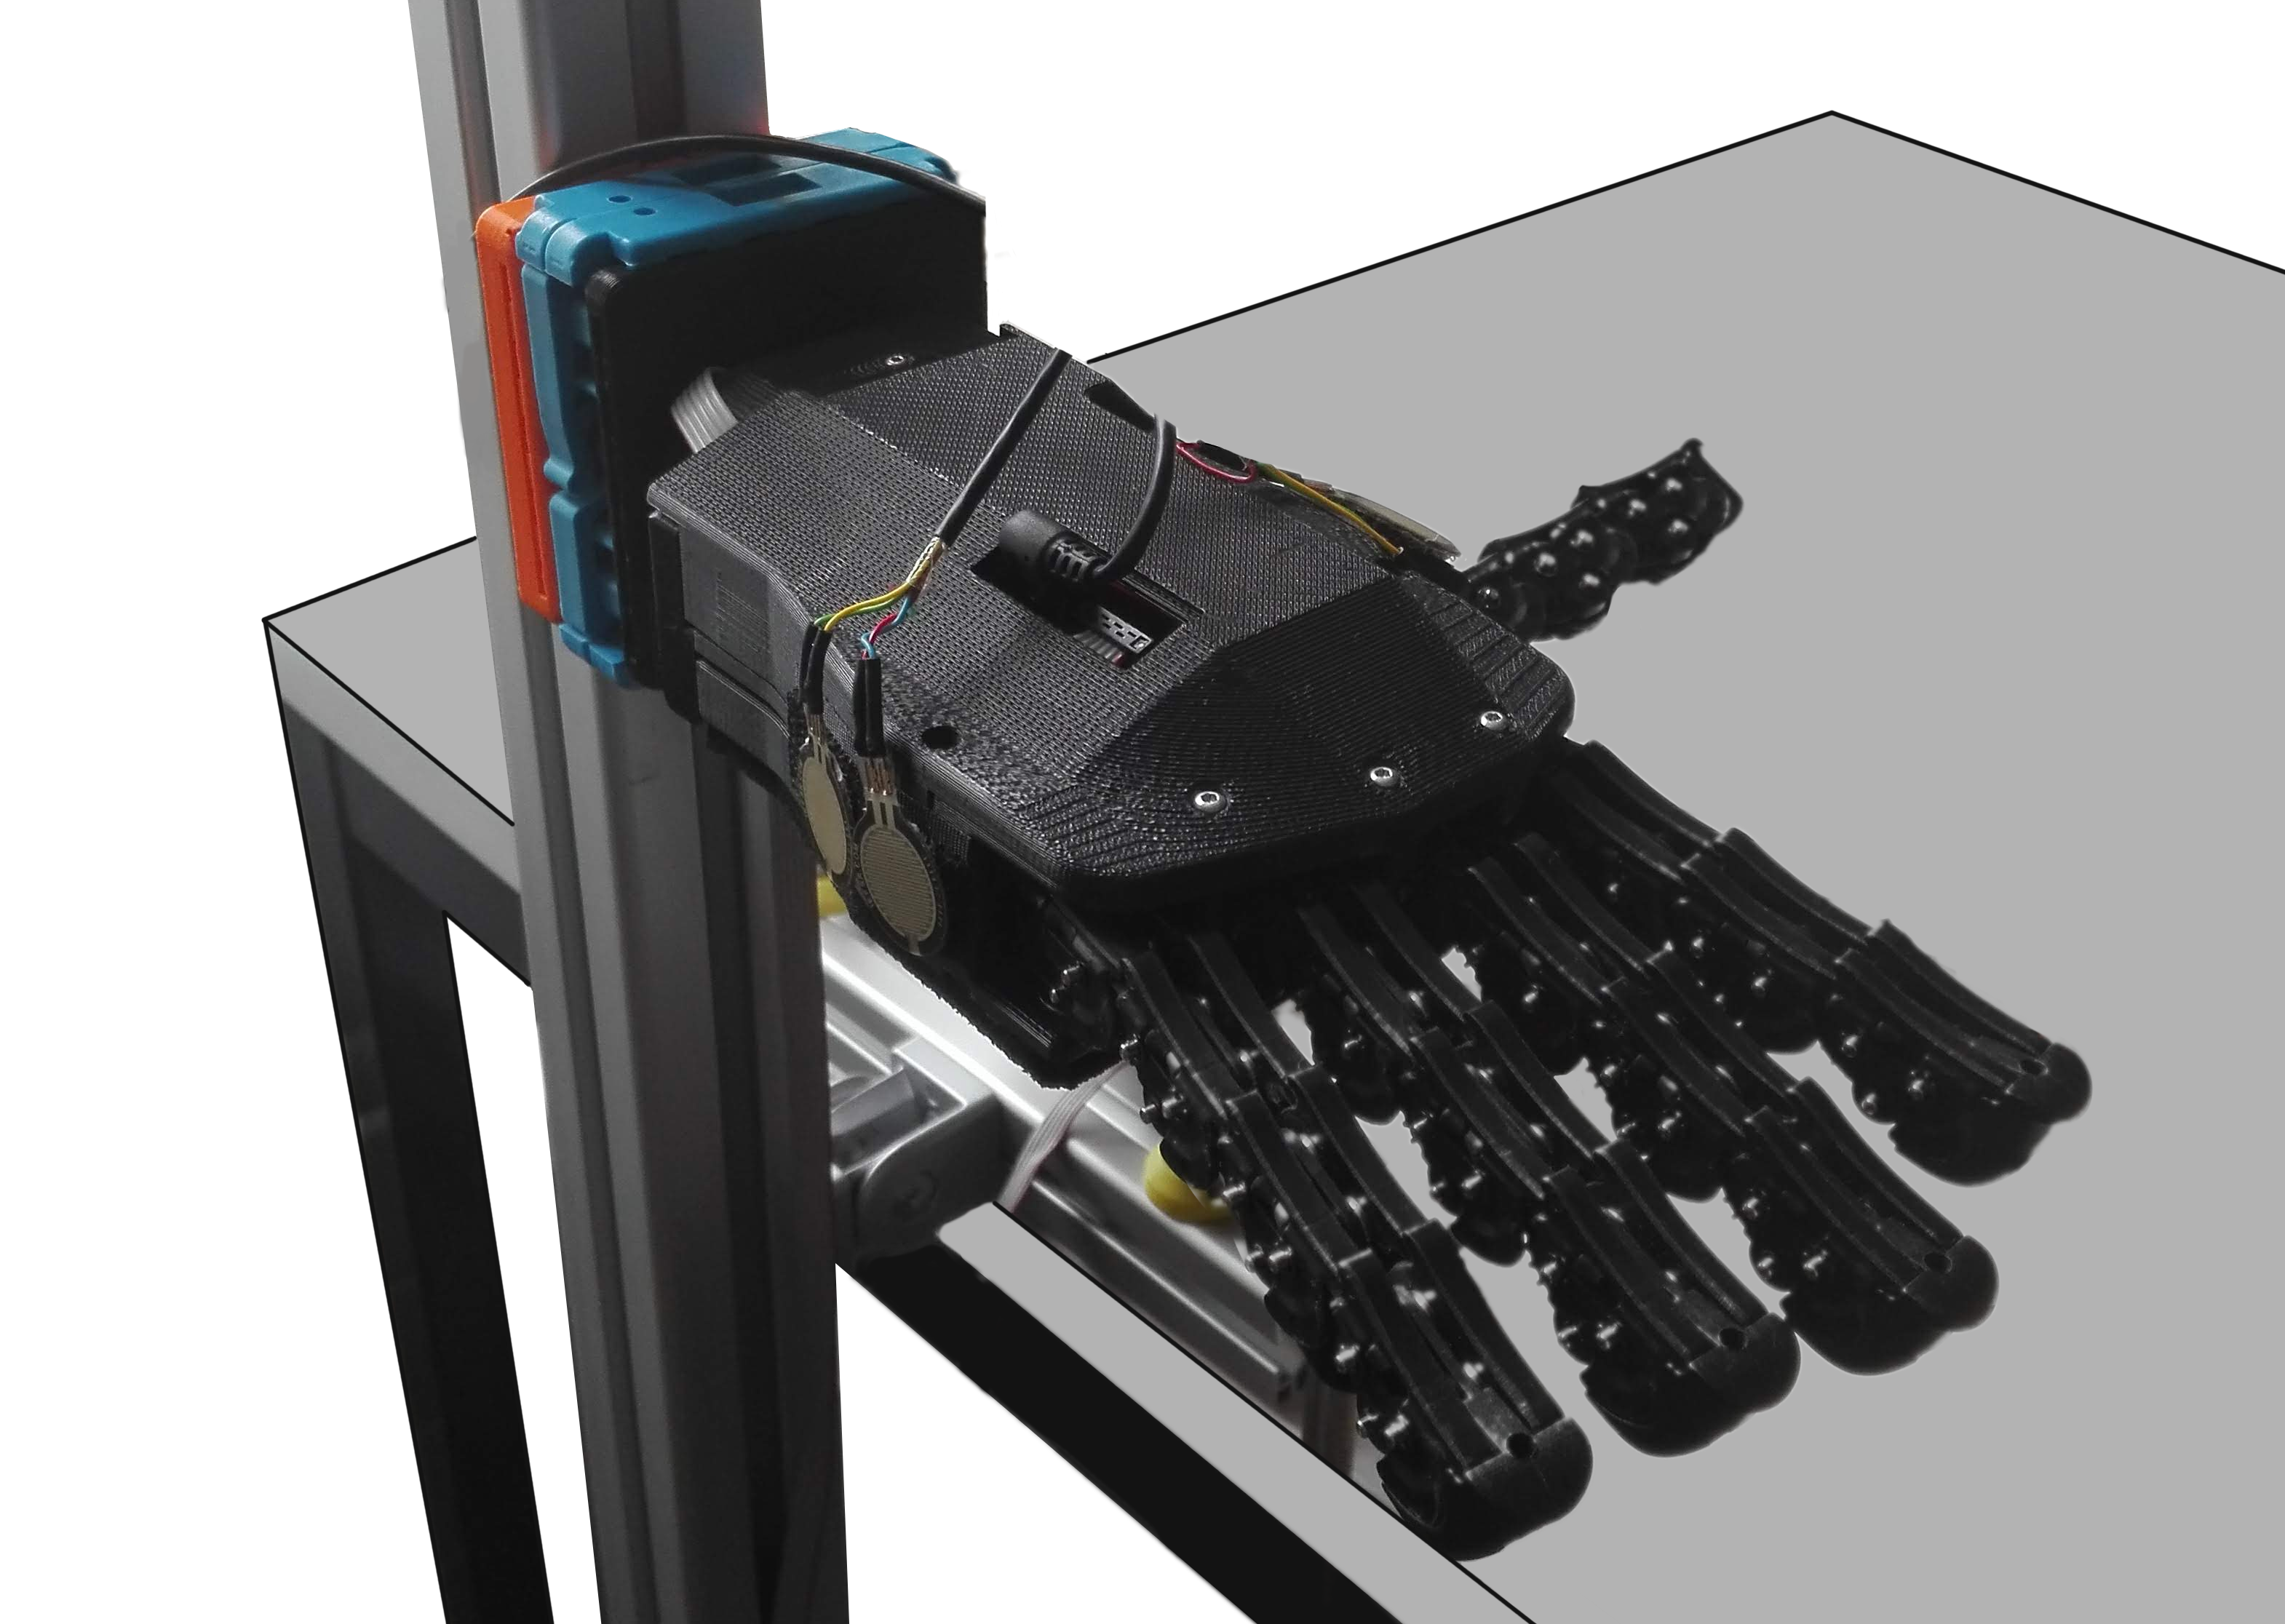
\includegraphics[width=0.6\textwidth]{Figure/stand.png}
\caption{Palm facing down environment}
\label{Fig:palmdown}
\end{figure}

\section*{Participants}\label{sec:participants}
The participants to the experiments have been selected in an heterogeneous fashion from male to female with ages in (24-35 years old). Although the hand sizes available for the experiments are considered sufficient, over bounding the ranges of the previous age set can provide interesting results.
This experimental part is looking for the existing of the relation above mentioned \ref{EQ:genericForce}, therefore it is providing the methodology approach to this problem.
Each participant is repeating each experiment five times, this provide useful information and allow to average the outcomes of the same participant.

\newpage
\section{Step input}
The simplest signal that can be sent to the Pisa/IIT SoftHand is a step signal on the reference position, in this way the participant's response can be evaluated. The step signal in this experiment is formally a shifted and scaled step signal, the transformation parameters have been chosen in order to start from a position without physical contact to a position where empirical experiments have shown a consistent contact. 
%The first three seconds of the experiment $q_0$ is sent, then $q_1$ is sent so that the whole experiment lasts 6 seconds.
\begin{equation}
Q_{r}(t)=\left\{\begin{matrix}
q_{0} & $ for $ & t < t_0 \\ 
q_{1} & $ for $ & t \geq t_0
\end{matrix}\right.
\label{EQ:StepSignal}
\end{equation}
%$$
%Q_r(t) =   
%\begin{cases} 
%k_0 & t < t_0\\
%k_1 & t \geq t_0
%\end{cases}
%$$
%with $k \in \mathbb{R}$.
\subsection{Description}
The parameters chosen for the experiment in order to go from a reference position where $F_h=0$ to a reference position where $F_h > 0$ are:
\begin{itemize}
\item $q_0 = 8000 $
\item $q_1 = 15000$
\item $t_0 = 3s$
\end{itemize}
the experiment lasts in total 6 seconds. A correlation between the reference position of the Pisa/IIT SoftHand and the values recorded from the FSRs is expected. The participants are applying a force ($F_{h}$) which is assumed to be proportional to the one applied from the robot to their hand during the handshake \ref{EQ:forceSteady}.
The same experiment has been executed with multiple participants, in order to increase the amount of data available for the model estimation. The values of reference position in this experiment $q_{0}$ and $q_{1}$, are fixed during multiple trials, therefore the participants are able to predict that at $t=t_0$ a higher reference signal is sent. Although, this behaviour has been considered not consistent to fit, in post processing, a model to the data, it can provide a first sight the relation $q$ vs. $F_h$.
%
%\textcolor{magenta}{insert unfiltered plot of q vs force}
%
%\begin{figure}[h]
%  \centering
%  \begin{minipage}[b]{0.4\textwidth}
%    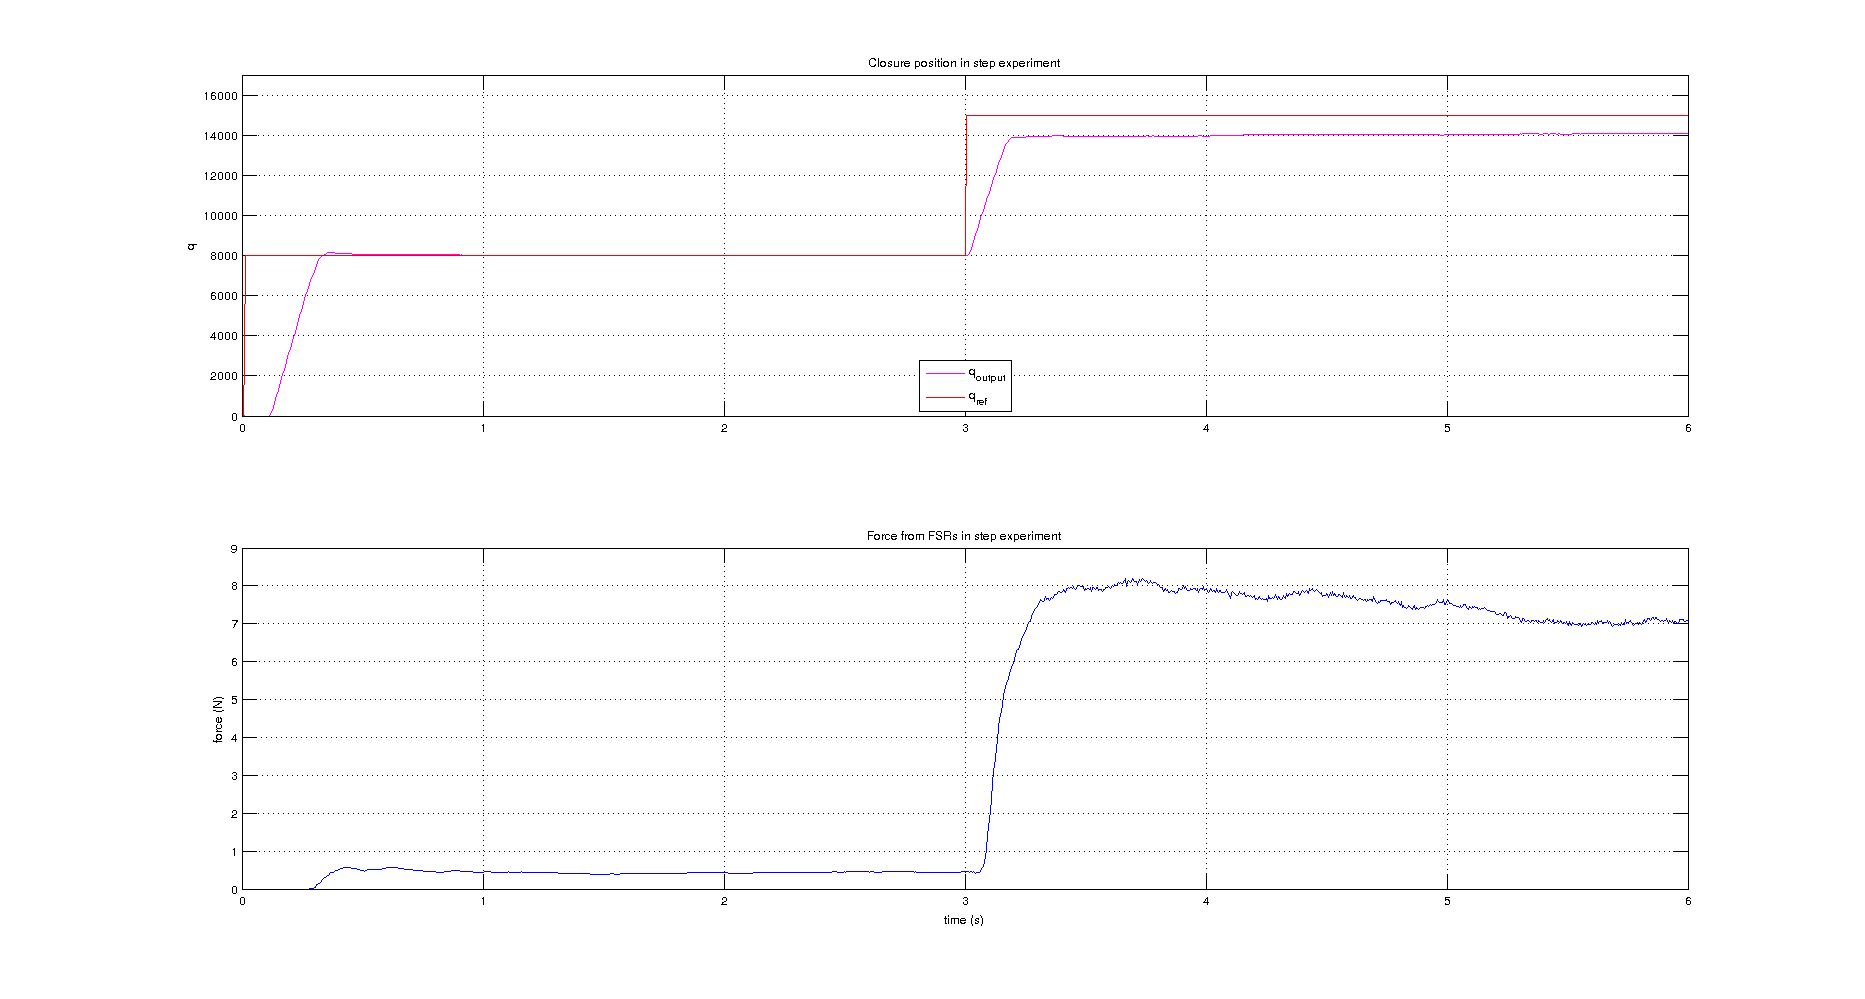
\includegraphics[width=\textwidth]{Figure/step.png}
%    \caption{Step experiment without transient}
%  \label{fig:step}
%  \end{minipage}
%  \hfill
%  \begin{minipage}[b]{0.4\textwidth}
%    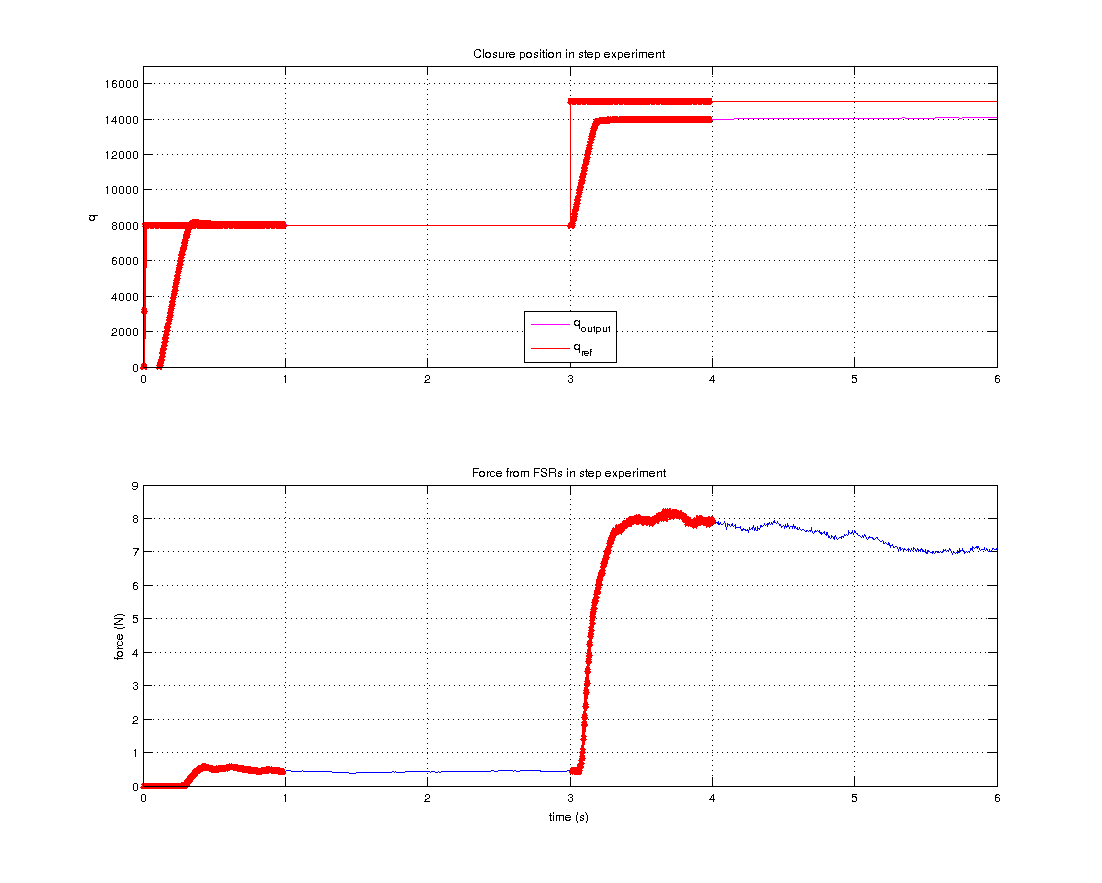
\includegraphics[width=\textwidth]{Figure/steptransient.png}
%    \caption{Step experiment with transient}
%    \label{Fig:steptransient}
%  \end{minipage}
%  %\caption{FSR sensors position on sensorized palm}
%\end{figure}
\begin{figure}[h]
\centering
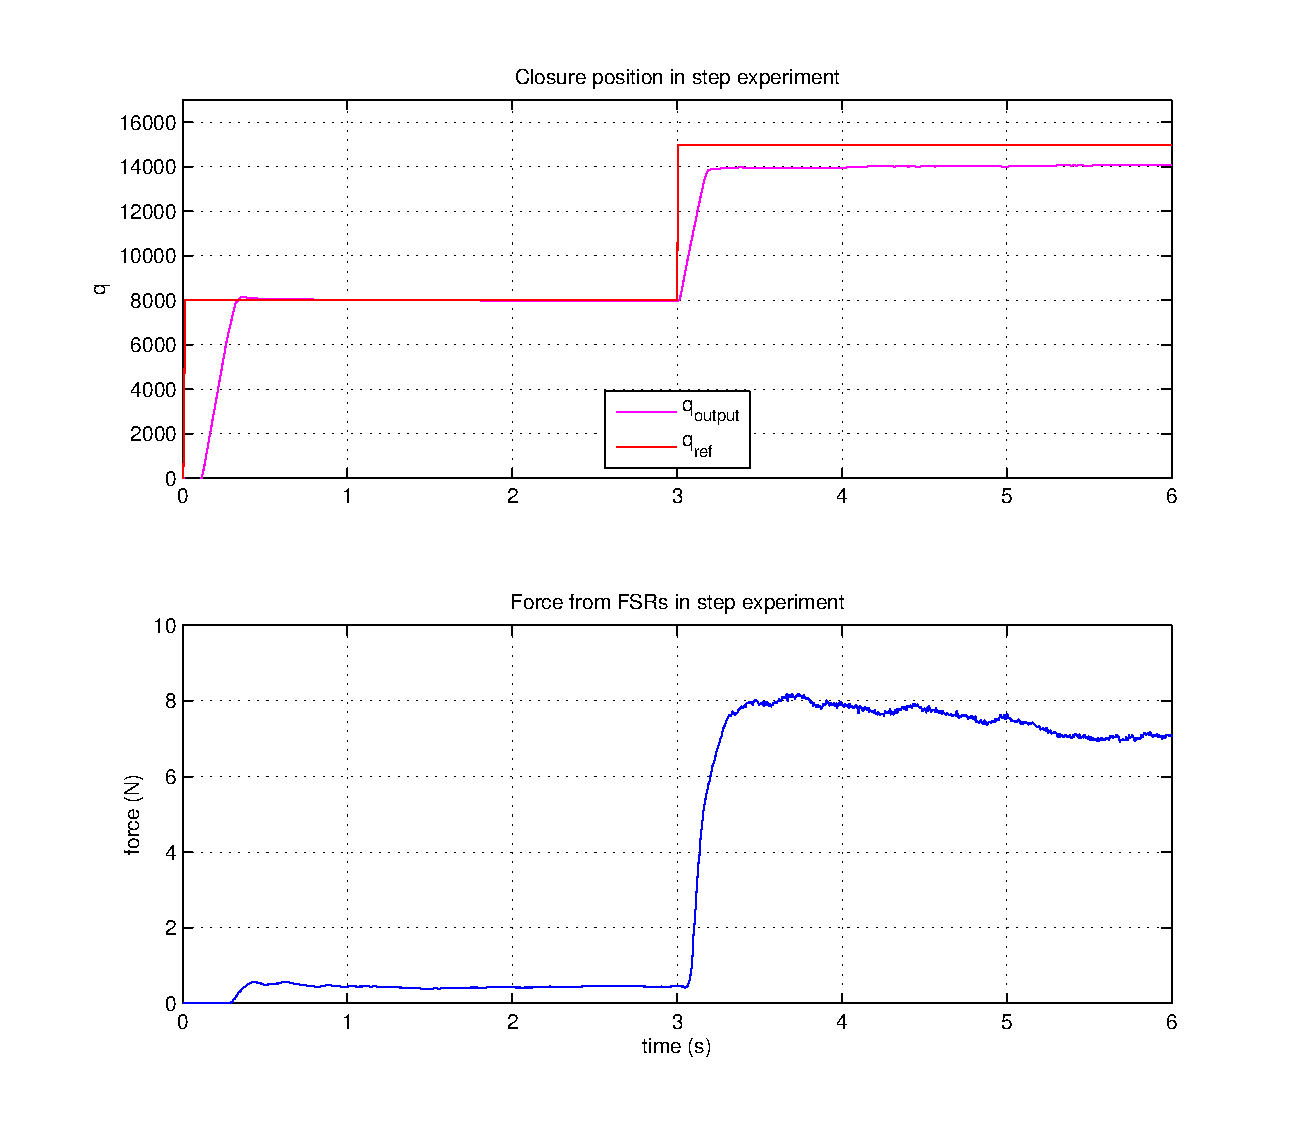
\includegraphics[width=0.7\textwidth]{Figure/step.eps}
  \caption{Step experiment in time}
  \label{Fig:step}
\end{figure}

%\textcolor{magenta}{insert step experiment plots force vs q}
\subsection{Transient filter}\label{sec:transientStep}
Giving as input to the system only two different values of reference position, makes more challenging to estimate a realistic model but it can already suggest that a correlation between $F_{h}$ and $q$ exists.
The Fig. \ref{Fig:step} shows the trend over the time of: $q_{ref}$, $q_{output}$ and the force $F_{h}$; clearly there are parts of these signals which are strictly related to the dynamics during the handshake. 
In order to filter these transient behaviours from the data a time slice has been selected to 1.0 second, which corresponds to $frac{1}{3}$ of total amount of time of each signal.
Removing the information of the time from the previous plots and comparing $q$ against the $F_{h}$ can provide an important information for selecting the correct transient window, \textit{noted as: TW}, in terms of standard deviation. \\


\begin{figure}[h]
  \centering
  \begin{minipage}[b]{0.4\textwidth}
    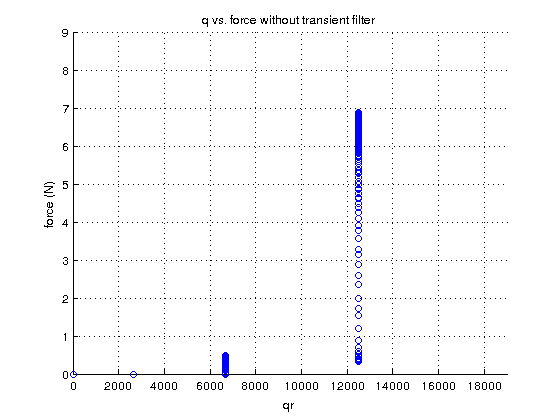
\includegraphics[width=\textwidth]{Figure/stepUnfilt.png}
    \caption{TW = 0}
  \label{Fig:qFUnfilt}
  \end{minipage}
  \hfill
  \begin{minipage}[b]{0.4\textwidth}
    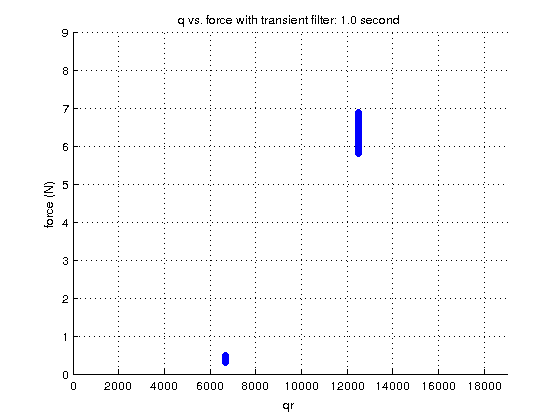
\includegraphics[width=\textwidth]{Figure/stepfilt.png}
    \caption{TW = 1s}
    \label{Fig:qFfilt}
  \end{minipage}
\caption{q vs. force comparing transient windows}
\label{Fig:qF}

\end{figure}

In \ref{Fig:qF} a comparison of the plot of $q$ vs. $F_{h}$ is shown, a transient window of 1.0 sec. is considered sufficient to reach the steady state grasping force. 
%\textcolor{magenta}{to justify better the choice of 1 second can be implemented a function calculating the standard deviation for each cut transient (too much?)}


\section{Pseudorandom input}\label{sec:pseudo}
The open loop experiment is trying to identify the relationship between robot closure position $q$ and the robot grasping force $F_{r}$. The procedure is to first find the relationship between $q$ and the force that the human apply on the sensors $F_{h}$ and lately using the assumption in \ref{EQ:forceSteady} to obtain $F_{r}$. 
The step experiment discussed in the previous section is a good starting point for an advanced study. 
As discussed in \ref{sec:participants}, experiments are repeated multiple times but the method allow the participants to understand the behaviour of the Pisa/IIT SoftHand and to predict the step signal amplitude. \\
An approach to solve this issue is to input to the device a random sequence of scaled-step signals, this avoid the participants to forecast the next $q$ of the Pisa/IIT SoftHand. A more advanced technique would be to either send a random sequence of scaled-steps and also to randomize the duration of each signal. This last approach can eventually provide more accurate results than the previous one, but the post processing of the data is expected to introduce issues for filtering the transient of each signal.
\subsection{Description}
The Pseudorandom input experiment is an open loop system where a sequence of steps, properly adapted to the range of admissible input closure signals $q$ as from \ref{EQ:qlimits}, is set as input to the Pisa/IIT SoftHand while the sensors are tracking the force $F_{h}$.
The reason behind a pseudo-randomized sequence is used, can be summarized in two important aspects:
\begin{itemize}
%\textcolor{magenta}{ CAN WE SAY THIS?}
\item participants are not able to forecast the next closure position $q$ and if each experiment is long enough, the order of each step signal is considered random,
%\item the steady state of $F_{h}( \hat{t} )$ for a certain $q(\hat{t})$ can be influenced $q(\hat{t}-1)$, and having a fully randomized sequence of $q$ can highlight this behaviour,
\item during the post processing procedure: having the exact same sequence of $q$ along multiple experiments allow to elaborate the data just using indexes.
\end{itemize}

\begin{figure}[h]
  \centering
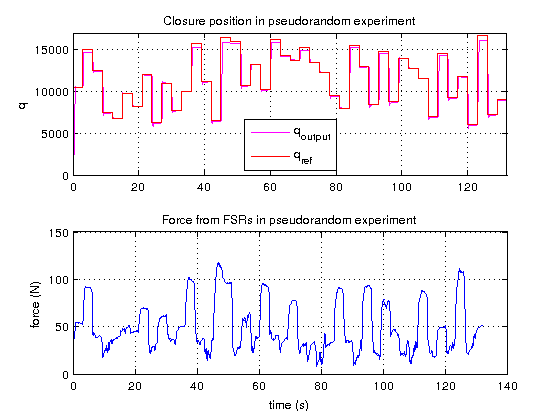
\includegraphics[width=0.7\textwidth]{Figure/pseudorandom_q.png}
  \caption{Pseudorandom experiment in time}
  \label{Fig:pseudo}
\end{figure}


A single experiment lasts 2'12", and the reference positions sent to the Device are randomized with a fixed seed and are unique, this means that if $\hat{q}$ is transmitted for the first time at $\hat{t}$ it is hold for 3 seconds and it won't be transmitted for the rest of the experiment.
Participants response can be evaluated in Fig. \ref{Fig:pseudoforce}, where the force $F_{h}$ during the experiment is plotted, these values are the average of the experiments between multiple participants where each participant repeated the same experiment 5 times.
The pseudorandom sequence given as input to the device is shown in \ref{Fig:pseudo}, in particular the plot contains $q_{ref}$ and $q_{output}$.\\
%
%\begin{figure}[h]
%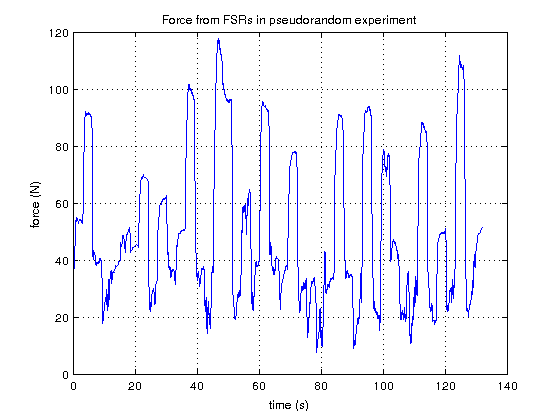
\includegraphics[width=\textwidth]{Figure/pseudoforce.png}
%  \caption{Pseudorandom experiment in time}
%  \label{Fig:pseudoforce}
%\end{figure}

\subsection{Transient filter}\label{sec:transientPseudo}
As for the one step experiment, a technique to filter the behaviours due to dynamics is needed; the same procedure described in \ref{sec:transient} is used and the transient window (TW) is set to 1.0 sec.
Comparing the values of $F_{h}$ and $q$ is beneficial to understanding how the human reacts to a robot handshaking. The prior expectation is that the higher the values of $q$ are and higher the force the human will apply on the Device, what it is still unknown is the type of relation between these two quantities. Let's set the TW = 1.0 sec. in post processing, remove the time information from  \ref{Fig:pseudo} and compare  $q$ vs. $F_{h}$.



\textcolor{magenta}{Insert plot q vs F; talk about the transient elaboration and explain how to find the model}
